\documentclass{beamer}
\usepackage[utf8]{inputenc}
\usepackage{graphicx}
\usepackage{hyperref}
\usepackage{url}
\usepackage[english]{babel}
\usepackage{tabu}
\usepackage{multirow}
\usepackage{amsmath}
\usepackage{color}
\usepackage{ulem}

\DeclareGraphicsExtensions{.pdf,.png,.jpg,.eps}

\newcommand{\todo}[1]{}
\renewcommand{\todo}[1]{{\color{red} TODO: {#1}}}

\newcommand*\mean[1]{#1} % no overrule in the slides

\usetheme{Frankfurt}

\title{Zombie Apocalypse}
\author{Adam Juraszek \and Ryan Leong Wei Shiong \and Matthew Signorini \and Ziying Yang}
\institute{The University of Melbourne}

\AtBeginSection[]
{
    \begin{frame}
        \frametitle{Table of Contents}
        \tableofcontents[currentsection]
    \end{frame}
    \stepcounter{subsection}
}

\begin{document}

\begin{frame}
    \titlepage
\end{frame}

\begin{frame}
    \frametitle{Table of Contents}
    \tableofcontents
\end{frame}

\section{SEIR Model}

\begin{frame}{SEIR Model}
    In terms of SEIR model:
    \begin{description}
        \item[Susceptible] Humans
        \item[Exposed] Infected
        \item[Infectious] Zombies
        \item[Recovered] Dead
    \end{description}

    \begin{center}
        \includegraphics[width=\textwidth]{model}
    \end{center}
\end{frame}

\begin{frame}{Infection}
    \begin{itemize}
        \item Probability of infection
        \item Infected are not contagious
        \item Infection takes 14 days on average.
        \item No recovery possible
    \end{itemize}
\end{frame} 

\begin{frame}{Zombies}
    \begin{itemize}
        \item Expected decomposition: 3 years
        \item No reproduction
        \item Slower movement
        \item Infectious
    \end{itemize}
\end{frame}

\section{World representation}

\begin{frame}{Mesh}
    \begin{itemize}
        \item 1D array with additional index
        \item has 2 cells wide border
    \end{itemize}

    \begin{center}
        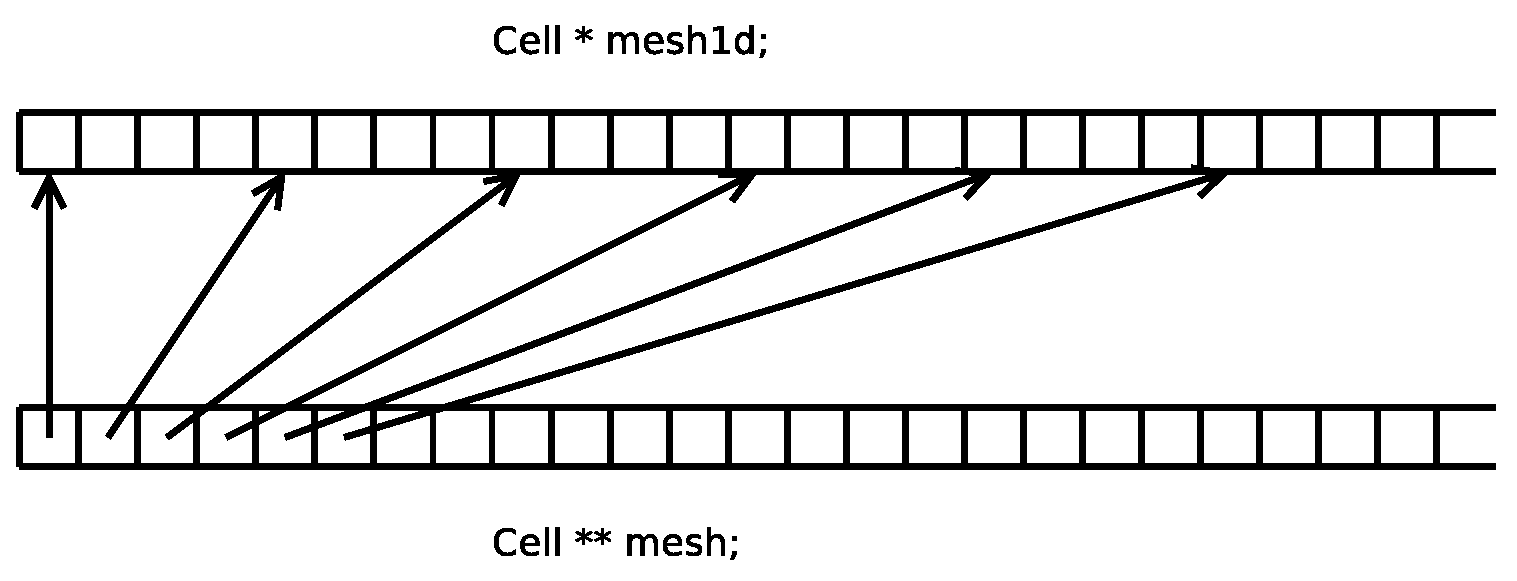
\includegraphics[width=0.8\textwidth]{mesh}
    \end{center}
\end{frame}

\begin{frame}{Borders}
    Borders have several uses:
    \begin{itemize}
        \item providing data for non-local processes
        \item transferring entities between worlds
    \end{itemize}
    \begin{columns}
        \begin{column}{.5\textwidth}
            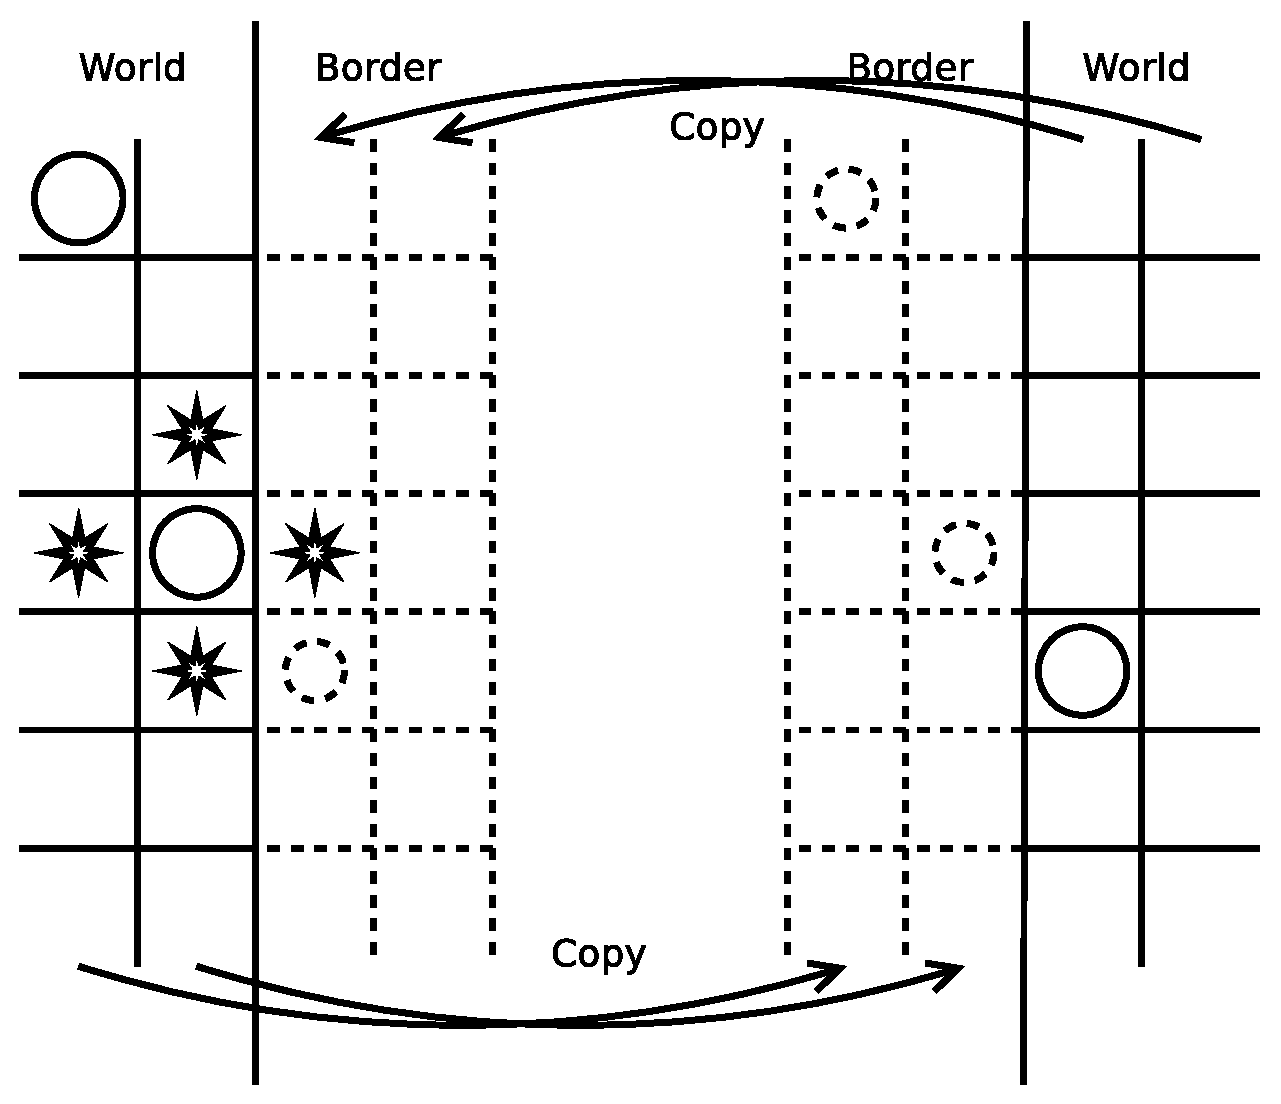
\includegraphics[width=0.9\textwidth]{border1}
        \end{column}
        \begin{column}{.5\textwidth}
            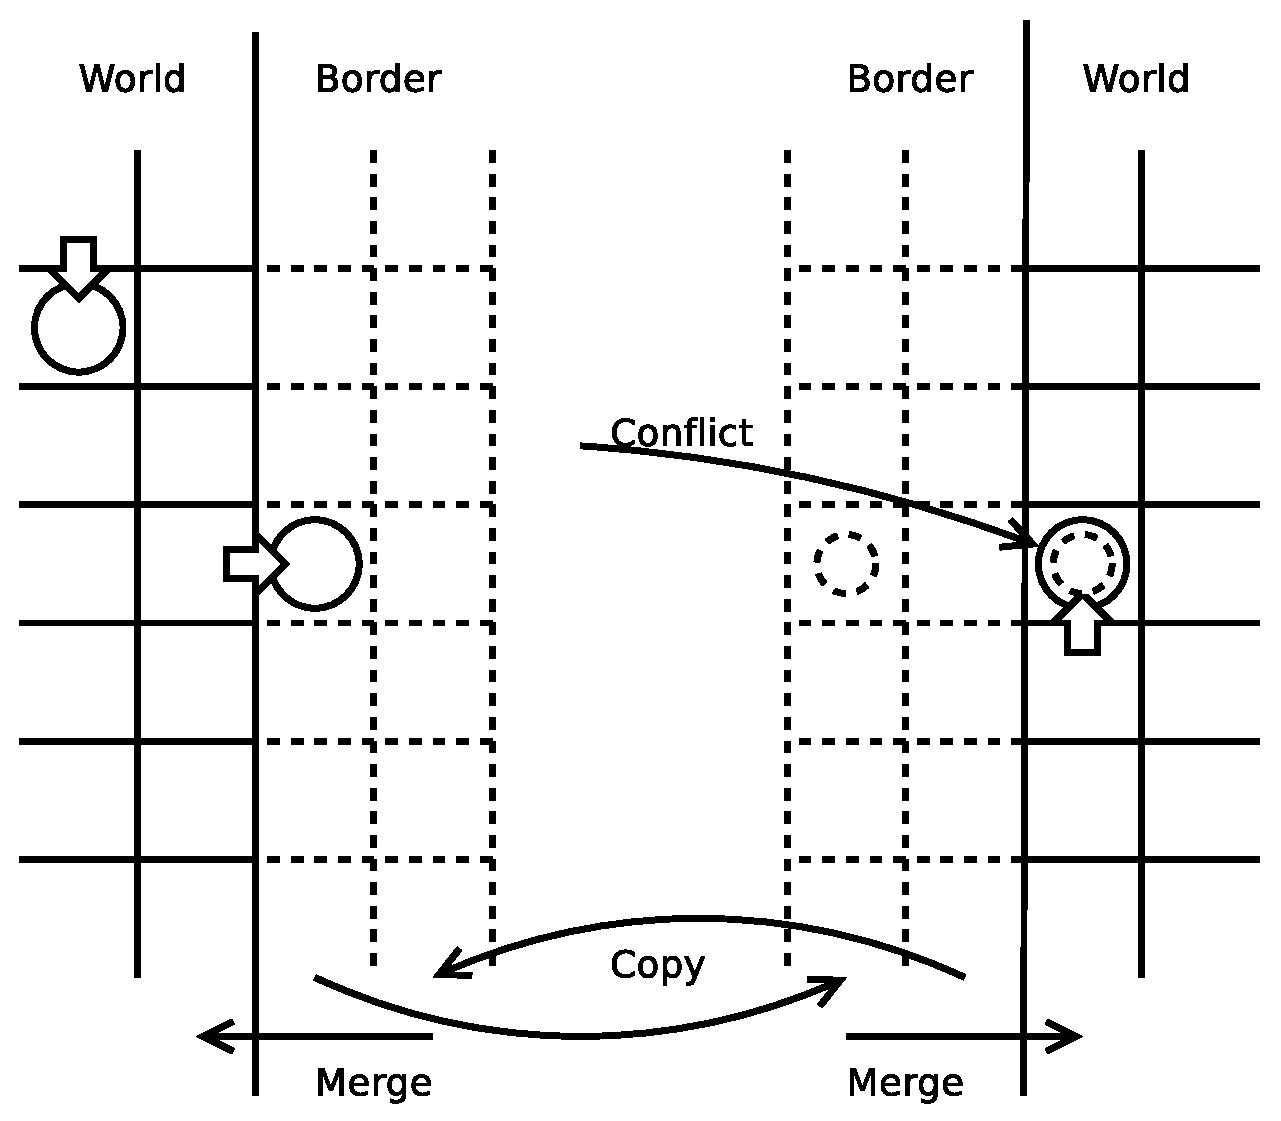
\includegraphics[width=0.9\textwidth]{border2}
        \end{column}
    \end{columns}
\end{frame}

\begin{frame}{Movement}
    \begin{columns}
        \begin{column}{.5\textwidth}
            \begin{itemize}
                \item Based on 12 surrounding cells
                \item Uses weighted sum of complex numbers
                \item Uses last move as inertia
                \item Speed is modeled as probability of movement
                \item Only moves if speed is sufficient
                \item Randomised; checking for alternatives
            \end{itemize}
        \end{column}
        \begin{column}{.5\textwidth}
            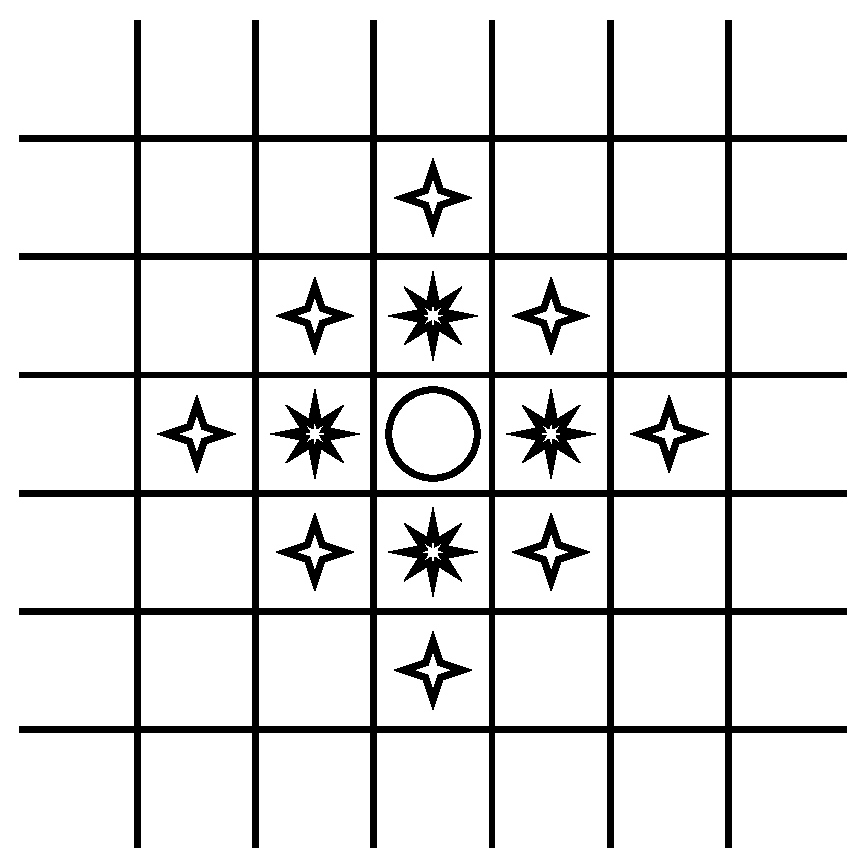
\includegraphics[width=0.9\textwidth]{movement}
        \end{column}
    \end{columns}
\end{frame}

\section{Humans}

\begin{frame}{Human Age Classes}
    \begin{itemize}
        \item According to Australia age structure and median age.
        \item Death probability and movement speed depend on age class.
    \end{itemize}

    \begin{block}{Age classes}
        \begin{description}[Middle age]
            \item[Child] 0--15
            \item[Young] 15--37.5
            \item[Middle age] 37.5--65
            \item[Elderly] 65+
        \end{description}
    \end{block}
\end{frame}

\begin{frame}{Human Death Rate}
    \begin{columns}
        \begin{column}{0.5\textwidth}
            Based on:
            \begin{itemize}
                \item mortality rates graph
                \item Gompertz–Makeham law
            \end{itemize}
        \end{column}
        \begin{column}{0.5\textwidth}
            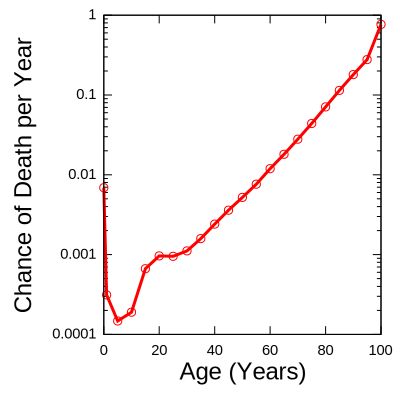
\includegraphics[width=0.9\textwidth]{USGompertzCurve}
        \end{column}
    \end{columns}
\end{frame}

\begin{frame}{Human Death Rate}{Probabilities}
    \begin{tabu} {| X[0.7,c,p] || X[0.7,c,p] | X[1.1,c,p] | X[0.9,c,p] | X[1,c,p] |}
        \rowfont{\bfseries}
        \hline
        Class Name &
        Age Range &
        Distribution &
        Average Death Rate (per~day) &
        Death Rate (per~day) \\
        \hline
        \hline
        \textbf{Child} & 0--15 & 18.2\% & \multirow{4}{*}{0.0017\%} & 0.00006\% \\
        \cline{1-3}\cline{5-5}
        \textbf{Young} & 15--37.5 & 31.8\% & & 0.00012\% \\
        \cline{1-3}\cline{5-5}
        \textbf{Middle Age} & 37.5--65 & 35.6\% & & 0.00096\% \\
        \cline{1-3}\cline{5-5}
        \textbf{Elderly} & 65+ & 14.4\% & & 0.0096\% \\
        \hline
    \end{tabu}

    $$ \mean{P(\text{Elder Death})} = 10\: \mean{P(\text{Middle Age Death})} $$
    $$ = 80\: \mean{P(\text{Young Death})} = 160\: \mean{P(\text{Child Death})} $$
\end{frame}

\begin{frame}{Human Death Rate}{Gender Difference}
    But females usually live longer than males.
    
    $$ DIFF = 82.4 / 78.5 = 1.0497 $$
    
    $$ P(\text{Male Child Death}) = 0.00006\% \cdot \sqrt{DIFF} $$
    $$ P(\text{Female Child Death}) = \frac{0.00006\%}{\sqrt{DIFF}} $$
    \ldots
\end{frame}

\begin{frame}{Human Sex Ratio}
    \begin{block}{Initialisation}
        $$ \text{Male} : \text{Female} = 0.5025 : 0.4975 $$
    \end{block}
    \begin{block}{Birth}
        $$ \text{Male Child} : \text{Female Child} = 0.5146 : 0.4854 $$
    \end{block}
\end{frame}

\begin{frame}{Human Fertility}
    \begin{block}{Fertile females}
        From: $15 \pm 2$\\
        To: $45 \pm 5$
    \end{block}
    \begin{block}{Fertile males}
        From: $15 \pm 2$\\
        To: $80 \pm 10$
    \end{block}
\end{frame}

\begin{frame}{Human Pregnancy}
    \begin{block}{Pregnancy duration}
        9 months $\pm$ 2 weeks
    \end{block}
    \begin{block}{Initially pregnant females}
        $$ P(\text{Pregnant Female in Fertility Period}) $$
        $$ = \frac{\text{average number of children per female life} \times \text{pregnancy duration}}{\text{average length of fertility period}} $$
        $$ = \frac{1.77 \times 9 (\text{months})}{30 (\text{years})} = 4.36\% $$
    \end{block}
\end{frame}

\begin{frame}{Human Reproduction}
    \begin{itemize}
        \item If male and female are at adjacent cells and both are fertile and female is not pregnant, they make love.
        \item Up to 3 children may be convieved with a certain probability.
        \item After pregnancy duration the child is born to an adjact cell.
        \item If no cell is free, the child stays in the womb until next day. 
    \end{itemize}
\end{frame}

\begin{frame}{Human Population}
    \begin{itemize}
        \item Initial density is $ \frac{0.17}{2} = 0.085 $
        \item The number of people depends on density and world size.
    \end{itemize}
\end{frame}

\section{Stability}

\begin{frame}{Stability Approaches}
    \begin{itemize}
        \item Human birth rate controlled by function dependent on desity.
        \item Multiple functions tried with various results.
        \item Probability of infection 1\% is always unstable.
        \item Probability changed to 0.75\%.
    \end{itemize}
\end{frame}

\begin{frame}{Uncontrolled}
    \begin{columns}
        \begin{column}{0.4\textwidth}
            \begin{itemize}
                \item Fixed probability of child birth
                \item Stable without zombies
                \item Unstable with zombies
                \item After about only 74 years zombies died out.
            \end{itemize}
        \end{column}
        \begin{column}{0.6\textwidth}
            \includegraphics[width=\textwidth]{uncontrolled_birth}
        \end{column}
    \end{columns}
\end{frame}

\begin{frame}{Equal}
    \begin{columns}
        \begin{column}{0.4\textwidth}
            \begin{itemize}
                \item Probability depenent on number of deaths and infected.
                \item Unstable with zombies
            \end{itemize}
        \end{column}
        \begin{column}{0.6\textwidth}
            \includegraphics[width=\textwidth]{equal_birth}
        \end{column}
    \end{columns}
\end{frame}

\begin{frame}{Density Dependent}{Linear}
    \begin{columns}
        \begin{column}{0.4\textwidth}
            \begin{itemize}
                \item The lower population density, the higher child birth probability.
                \item $Ratio = \frac{\text{Initial density}}{\text{Current density}}$
                \item $Prob' = Prob \cdot Ratio$
                \item Not strong enough
            \end{itemize}
        \end{column}
        \begin{column}{0.6\textwidth}
            \includegraphics[width=\textwidth]{density_birth}
        \end{column}
    \end{columns}
\end{frame}

\begin{frame}{Density Dependent}{Power of density ratio}
    \begin{columns}
        \begin{column}{0.4\textwidth}
            \begin{itemize}
                \item Power of density ratio
                \item Functions:
                    \begin{enumerate}
                        \item $ Ratio^{Ratio \cdot const} $
                        \item \sout{$Ratio^{const}$}
                    \end{enumerate}
                \item Situation Awareness Coeficient: $Const = 2.5$
            \end{itemize}
        \end{column}
        \begin{column}{0.6\textwidth}
            \includegraphics[width=\textwidth]{fertilisation_probability}
        \end{column}
    \end{columns}
\end{frame}

\begin{frame}{Density Dependent}{Results}
    \begin{center}
        \only<1>{\includegraphics[width=0.9\textwidth]{stable}}
        \only<2>{\includegraphics[width=0.9\textwidth]{stable_1000000}}
    \end{center}
\end{frame}

\section{Results}

\begin{frame}
    \todo{Demographics and scaling for 500 by 500}
\end{frame}

\section{Larger results}

\begin{frame}
    \todo{Scaling using OpenMP and MPI}
\end{frame}

\section{Planet}

\begin{frame}{Planet}
    \begin{columns}
        \begin{column}{0.4\textwidth}
            \begin{itemize}
                \item Simulation of toroidal planet
                \item Size: $8192 \times 4096$ on 128 nodes ($512 \times 512$ each) with 32 threads
                \item Run-time: 2 hours
                \item Simulated 1613 years (588745 days)
                \item Produced 64 GB of data
            \end{itemize}
        \end{column}
        \begin{column}{0.6\textwidth}
            \includegraphics[width=\textwidth]{torus/planet.pdf}
        \end{column}
    \end{columns}
\end{frame}

\begin{frame}{Planet after 6 years}
    \begin{center}
        \only<1>{\includegraphics[width=\textwidth]{torus/step-002190-torus.png}}
        \only<2>{\includegraphics[width=0.9\textwidth]{step-002190.pdf}}
    \end{center}
\end{frame}

\begin{frame}{Planet after 19 years}
    \begin{center}
        \only<1>{\includegraphics[width=\textwidth]{torus/step-006935-torus.png}}
        \only<2>{\includegraphics[width=0.9\textwidth]{step-006935.pdf}}
    \end{center}
\end{frame}

\begin{frame}{Planet after 46 years}
    \begin{center}
        \only<1>{\includegraphics[width=\textwidth]{torus/step-016790-torus.png}}
        \only<2>{\includegraphics[width=0.9\textwidth]{step-016790.pdf}}
    \end{center}
\end{frame}

\begin{frame}{Planet after 116 years}
    \begin{center}
        \only<1>{\includegraphics[width=\textwidth]{torus/step-042340-torus.png}}
        \only<2>{\includegraphics[width=0.9\textwidth]{step-042340.pdf}}
    \end{center}
\end{frame}

\begin{frame}{Planet after 162 years}
    \begin{center}
        \only<1>{\includegraphics[width=\textwidth]{torus/step-059130-torus.png}}
        \only<2>{\includegraphics[width=0.9\textwidth]{step-059130.pdf}}
    \end{center}
\end{frame}

\begin{frame}{Planet after 231 years}
    \begin{center}
        \only<1>{\includegraphics[width=\textwidth]{torus/step-084315-torus.png}}
        \only<2>{\includegraphics[width=0.9\textwidth]{step-084315.pdf}}
    \end{center}
\end{frame}

\begin{frame}{Planet after 251 years}
    \begin{center}
        \only<1>{\includegraphics[width=\textwidth]{torus/step-091615-torus.png}}
        \only<2>{\includegraphics[width=0.9\textwidth]{step-091615.pdf}}
    \end{center}
\end{frame}

\begin{frame}{Planet after 355 years}
    \begin{center}
        \only<1>{\includegraphics[width=\textwidth]{torus/step-129575-torus.png}}
        \only<2>{\includegraphics[width=0.9\textwidth]{step-129575.pdf}}
    \end{center}
\end{frame}

\begin{frame}{Planet after 1268 years}
    \begin{center}
        \only<1>{\includegraphics[width=\textwidth]{torus/step-462820-torus.png}}
        \only<2>{\includegraphics[width=0.9\textwidth]{step-462820.pdf}}
    \end{center}
\end{frame}

\begin{frame}{Planet after 1613 years}
    \begin{center}
        \only<1>{\includegraphics[width=\textwidth]{torus/step-588745-torus.png}}
        \only<2>{\includegraphics[width=0.9\textwidth]{step-588745.pdf}}
    \end{center}
\end{frame}

\section{Issues}

\begin{frame}{Directed movement}
    \begin{block}{Problem}
        \begin{itemize}
            \item When processing the world from left to right and from top to bottom.
            \item Entities cluster at right and bottom border.
        \end{itemize}
    \end{block}
    \begin{block}{Solution}
        \begin{itemize}
            \item Randomisation of processing order
        \end{itemize}
    \end{block}
\end{frame}

\begin{frame}{Border collisions}
    \begin{block}{Problem}
        \begin{itemize}
            \item When using MPI
            \item Movement depend on input and output world.
            \item Output world is not available for border.
        \end{itemize}
    \end{block}
    \begin{block}{Possible Solution}
        \begin{itemize}
            \item Strict ordering and locking
            \item Processing the border by both nodes
            \item Requires random number generator synchronisation, processing order synchronisation
            \item Not implemented
        \end{itemize} 
    \end{block}
\end{frame}

\begin{frame}{Data processing}
    \begin{block}{Problem}
        \begin{itemize}
            \item There are thousands of files generated.
            \item Total size is tens of GigaBytes.
        \end{itemize}
    \end{block}
    \begin{block}{Solution}
        \begin{itemize}
            \item Automatisation by support programs and scripts.
        \end{itemize}
    \end{block}
\end{frame}

\begin{frame}{Data processing}{Schema}
    \begin{center}
        % left, bottom, right, top
        \only<1>{\includegraphics[trim=0 445 0 0,clip,width=0.7\textwidth]{toolchain}}
        \only<2>{\includegraphics[trim=0 0 0 370,clip,width=0.7\textwidth]{toolchain}}
    \end{center}
\end{frame}

\section{Questions}

\begin{frame}{Conclusion}
    \huge{Questions?}
\end{frame}

\end{document}
